% !TeX spellcheck = ru_RU
% !TEX root = vkr.tex

\section{Обзор}
\label{sec:relatedworks}
% \emph{Обзор должен быть.} 
% Здесь нужно писать, что индустрия и наука уже сделали по вашей теме. Он нужен, чтобы Вы случайно не изобрели какой-нибудь велосипед.

%\subsection{Особенности процесса разработки под ПЛИС}
%Программируемые логические интегральные схемы (ПЛИС) -- это особый вид микросхем, логика которых не определяется на этапе производства, а задается инженером путем её программирования. ПЛИС состоит из набора логических блоков и множества программируемых соединений. Логические блоки содержат примитивы, такие как: D-триггеры, таблицы перекодировки (LUT), DSP-блоки, мультиплексоры, порты ввода-вывода, блоки памяти. 
%
%Важно отметить, что процесс программирования ПЛИС отличается от процесса программирования процессора в силу того, что ПЛИС, в отличие от процессора, не исполняет написанный под нее код. В случае ПЛИС код, написанный на языке описания аппаратуры (Hardware Description Language, HDL) конфигурирует соединения между внутренними примитивами, обеспечивая заданную алгоритмику работы.
%
%Для программирования ПЛИС используются предоставляемые её производителем программатор и IDE. Основной задачей IDE является преобразование HDL-кода в набор примитивов, имеющихся в ПЛИС, их коммутация и размещение на ПЛИС. В связи с этим основными компонентами IDE являются: редактор HDL-кода, синтезатор, оптимизатор размещения и маршрутизации. Разработчик может оказывать влияние на синтезатор и оптимизатор при помощи ограничений (constraints).
%
%Результатом разработки на языках HDL являются готовые функциональные блоки, называемые IP-ядрами. IP-ядро может использоваться как самостоятельно, так и входить в состав более сложных ядер. На основе IP-ядра может быть получена интегральная схема специального назначения (ASIC), которая впоследствии может быть поставлена на серийное производство.
%
%В настоящее время ПЛИС зачастую комбинируют вместе с процессором на одном общем кристалле, получая систему на кристалле (System-on-Chip, SoC). Такая система состоит из двух подсистем: процессорной системы (PS) и программируемой логики (PL). Взаимодействие между подсистемами осуществляется по стандартизированным интерфейсам. Также SoC оснащён разнообразной периферией, которая позволяет организовывать эффективное взаимодействие с таким устройством, например, в целях отладки. Мощностей процессорной системы достаточно для развертывания операционной системы Linux\cite{linaro_linux, xilinx_linux}. Если наличие ОС избыточно, то процессорная система может быть использована для развертывания Bare-Metal приложений. Наличие процессорной системы расширяет возможности по использованию ПЛИС и существенно упрощает отладку разрабатываемых IP-ядер. В связи с этим одним из сценариев использования систем на кристалле является организация платформ для разработки, отладки и апробации IP-ядер.

\subsection{Особенности процесса разработки под ПЛИС}

Программируемые логические интегральные схемы (ПЛИС) -- это класс цифровых интегральных схем, логика которых не определяется на этапе производства, а конфигурируется пользователем после изготовления. ПЛИС состоит из набора логических блоков и множества программируемых соединений. Логические блоки содержат примитивы, такие как: D-триггеры, таблицы перекодировки (Lookup Table, LUT), DSP-блоки, мультиплексоры, порты ввода-вывода и блоки памяти. 

Важно отметить, что процесс разработки для ПЛИС существенно отличается от процесса программирования процессора, поскольку ПЛИС, в отличие от процессора, не выполняет последовательность инструкций. В случае ПЛИС код, написанный на языке описания аппаратуры (Hardware Description Language, HDL), описывает структуру и поведение цифровой схемы. На основе данного описания инструменты автоматизированного проектирования формируют конфигурацию внутренних ресурсов микросхемы, обеспечивающую реализацию заданного алгоритма.

Для разработки под ПЛИС используются программные средства, предоставляемые производителем микросхемы. Современные средства разработки включают интегрированную среду проектирования (IDE), обеспечивающую полный цикл проектирования. Основной задачей такой среды является преобразование HDL-кода в конфигурацию логических примитивов, имеющихся в ПЛИС, их размещение и маршрутизация соединений. В связи с этим основными компонентами IDE являются: редактор HDL-кода, синтезатор, средство размещения и трассировки (place-and-route), а также генератор конфигурационного файла (битового потока). Разработчик может оказывать влияние на синтез и размещение при помощи ограничений (constraints), задающих временные, топологические и электрические параметры проекта.

Результатом разработки на языках HDL является описание аппаратной структуры, которое может быть оформлено в виде повторно используемых модулей, называемых IP-ядрами. IP-ядро может использоваться как самостоятельно, так и входить в состав более сложных систем. При необходимости RTL-описание проекта может быть использовано в дальнейшем для разработки интегральной схемы специального назначения (Application-Specific Integrated Circuit, ASIC), предназначенной для серийного производства.

В настоящее время ПЛИС зачастую комбинируются с процессорным ядром на одном кристалле, образуя систему на кристалле (System-on-Chip, SoC). Такая система состоит из двух основных подсистем: процессорной системы (Processing System, PS) и программируемой логики (Programmable Logic, PL). Взаимодействие между подсистемами осуществляется по стандартизированным интерфейсам (например, AXI). Наличие процессорной подсистемы позволяет выполнять высокоуровневое управление, конфигурацию и отладку аппаратных модулей. Производительности процессорной системы, как правило, достаточно для развертывания операционной системы Linux\cite{linaro_linux, xilinx_linux}. При отсутствии необходимости использования полноценной операционной системы возможно создание приложений типа Bare-Metal. Интеграция процессорной системы и программируемой логики расширяет функциональные возможности устройства и упрощает процесс верификации и отладки разрабатываемых аппаратных модулей. В связи с этим одним из распространённых сценариев применения SoC является организация платформ для разработки, отладки и апробации IP-ядер.


\subsection{Используемые технологии}

\subsubsection{Платформа}

Задачей разрабатываемого обнаружителя является обнаружение радиосигналов в заданном диапазоне частот и оценка их параметров. Для функционирования обнаружителя требуется входной цифровой сигнал, сформированный на основе принимаемого радиочастотного сигнала. Следовательно, аппаратная платформа должна обеспечивать не только вычислительные ресурсы ПЛИС, но и средства радиочастотного приёма и аналого-цифрового преобразования.

Таким образом, для реализации системы обнаружения требуется устройство, включающее систему на кристалле (SoC) и радиочастотный приёмопередающий тракт. Подобные устройства относятся к классу программно определяемых радиосистем (Software Defined Radio, SDR), в которых значительная часть обработки сигнала выполняется программно или аппаратно-программными средствами.

В качестве аппаратной платформы была выбрана модифицированная версия устройства ADALM-PLUTO (Pluto SDR+), в которой посредством изменения конфигурации расширен рабочий диапазон частот с 325~МГц--3{,}8~ГГц до 70~МГц--6~ГГц. Данное устройство сочетает в себе вычислительные ресурсы и радиочастотный тракт и обладает оптимальным соотношением стоимости и функциональных возможностей для решения поставленной задачи.


Основными компонентами выбранной платформы являются:
\begin{itemize}
	\item система на кристалле AMD Zynq-7000 SoC, включающая процессорную подсистему и программируемую логическую часть;
	\item микросхема приемопередатчика AD9363\cite{ad9363}, представляющая собой интегрированный RF-трансивер со встроенными аналого-цифровыми и цифро-аналоговыми преобразователями и цифровым интерфейсом передачи I/Q-отсчётов.
\end{itemize}


\subsubsection{Используемые инструменты}

При разработке проектов для ПЛИС выбор инструментов во многом определяется производителем целевой микросхемы. Как отмечалось ранее, код, написанный на языках HDL, не исполняется непосредственно устройством, а представляет собой описание структуры и поведения разрабатываемой цифровой схемы. На основе данного описания формируется конфигурация аппаратных ресурсов ПЛИС.

Преобразование RTL-описания в технологически зависимое представление, состоящее из примитивов целевой архитектуры, выполняется инструментом синтеза. Процесс синтеза требует информации о составе и характеристиках ресурсов выбранной ПЛИС. После этапа синтеза выполняются процедуры размещения (placement) и трассировки (routing), а также статический временной анализ (Static Timing Analysis), позволяющий проверить корректность работы схемы с учётом заданных временных ограничений. Все перечисленные этапы требуют детального знания архитектуры устройства, поэтому официальные средства разработки предоставляются производителем ПЛИС.

В рассматриваемой работе используется система на кристалле семейства Zynq-7000, разработанная компанией AMD (ранее Xilinx). В качестве основной среды аппаратного проектирования применяется пакет Vivado Design Suite\cite{vivado}, предназначенный для синтеза, реализации и генерации конфигурационного файла. 

Поскольку используемая платформа представляет собой SoC с процессорной подсистемой на базе ARM, для разработки программного обеспечения на языках C и C++ и его последующей загрузки и отладки используется среда AMD Vitis Unified Software Platform\cite{vitis}.

В качестве языка описания аппаратуры (Hardware Description Language, HDL) могут использоваться VHDL\cite{vhdl}, Verilog\cite{verilog} и SystemVerilog\cite{system_verilog}, которые получили широкое распространение в промышленной практике. Среда Vivado поддерживает данные языки. Для реализации обнаружителя в рамках данной работы был выбран язык VHDL, поскольку в организации АО концерн \enquote{ГРАНИТ} данный язык является основным.


\subsection{Существующие решения}

Разработанные IP-ядра зачастую обладают высокой коммерческой ценностью, поскольку на их основе могут быть созданы серийно производимые интегральные схемы. В силу этого значительная часть промышленных IP-ядер распространяется на проприетарной основе и недоступна для свободного использования и модификации. 

В то же время существуют проекты и сообщества, разрабатывающие IP-ядра с открытым исходным кодом. К числу таких ресурсов относятся специализированные каталоги и репозитории, например OpenCores\cite{opencores_home}, FuseSoC\cite{fusesoc_dir}, а также агрегированные коллекции VHDL/Verilog IP-ядер\cite{ip_cores_collection}. Подобные решения, как правило, ориентированы на реализацию базовых интерфейсов, периферийных контроллеров или типовых функциональных блоков и могут иметь ограничения по уровню оптимизации, поддержке и адаптации под конкретные аппаратные платформы.

Дополнительно необходимо учитывать, что IP-ядро может быть реализовано с использованием вендор-специфичных примитивов и библиотек, что приводит к его несовместимости с ПЛИС другого производителя. Хотя RTL-описание в общем случае является переносимым, практическая реализация часто зависит от доступных аппаратных ресурсов, таких как блоки памяти, DSP-модули или специализированные интерфейсы. Возможен также сценарий, при котором IP-ядро не может быть реализовано на младших моделях ПЛИС того же семейства из-за недостаточного объёма доступных ресурсов.

Каждый из перечисленных факторов может служить обоснованием необходимости разработки собственного IP-ядра. В данной работе рассматривается создание собственного IP-ядра обнаружителя для платформы AMD Zynq-7000 SoC\cite{zynq7000}, поскольку проведённый обзор доступных открытых IP-ядер показал отсутствие готовых реализаций обнаружителя.




\subsection{Корреляционное обнаружение сигналов}

При обнаружении сигналов широко применяется подход, основанный на использовании преамбулы — заранее известной последовательности отсчётов, обладающей хорошими автокорреляционными свойствами. 

Приёмник выполняет сравнение принятого сигнала с опорной преамбулой посредством вычисления взаимнокорреляционной функции, которая количественно характеризует степень сходства двух сигналов~\cite{sergienko_dsp}.

Взаимнокорреляционная функция для дискретных сигналов может быть записана в виде
\begin{equation}
	R_{xy}(k) = \sum_{n=0}^{N-1} x(n)\, y^*(n-k),
\end{equation}
где $x(n)$ — принятый сигнал, $y(n)$ — опорная преамбула, $(\cdot)^*$ обозначает комплексное сопряжение, $N$ — длина преамбулы.

При наличии сигнала максимум взаимнокорреляционной функции существенно превышает уровень отклика, формируемого шумом, что позволяет судить о наличии сигнала и его временном положении. Амплитуда корреляционного пика пропорциональна энергии сигнала.

Введём две гипотезы:
\[
H_0: x(n) = w(n),
\]
\[
H_1: x(n) = s(n) + w(n),
\]
где $w(n)$ — аддитивный белый гауссовский шум, $s(n)$ — искомый сигнал.

Решение об обнаружении принимается по правилу
\begin{equation}
	\max_k |R_{xy}(k)| 
	\mathop{\gtrless}_{H_0}^{H_1} \gamma,
\end{equation}
где $\gamma$ — порог обнаружения, выбираемый исходя из допустимой вероятности ложного срабатывания.

В отсутствии сигнала отклик корреляционного обнаружителя представляет собой случайную величину с известным распределением, что позволяет задать порог $\gamma$ в соответствии с требуемой вероятностью ложной тревоги.

Корреляционный обнаружитель является оптимальным для канала с аддитивным белым гауссовским шумом при известной форме сигнала~\cite{black_book}. 
По этой причине в работе рассматривается разработка корреляционного обнаружителя.

Принятый радиосигнал отличается от переданного вследствие воздействия шумов приёмного тракта, внешних помех, эффектов многолучевого распространения, а также нестабильности опорных генераторов передающей и приёмной сторон.

Поскольку корреляционный обнаружитель основан на когерентном суммировании отсчётов, наличие частотного рассогласования $\Delta f$ между сигналом и опорой приводит к фазовому вращению во времени и снижению амплитуды корреляционного пика (рис. 1). 

Поиск частотного смещения осуществляется дискретным перебором в пределах заранее известного диапазона. Непрерывный перебор невозможен, поэтому диапазон частот дискретизируется с некоторым шагом $\Delta f_{step}$.

Величина шага связана с длительностью преамбулы. Чем больше длина преамбулы, тем уже главный лепесток функции неопределённости и тем меньше допустимая остаточная частотная ошибка. 

Если шаг перебора слишком велик, остаточная частотная ошибка может привести к снижению корреляционного пика ниже порогового уровня и, как следствие, к пропуску сигнала. С другой стороны, уменьшение шага увеличивает число вычислительных операций и требования к вычислительным ресурсам.

\begin{figure}[h]
	\caption{Влияние частотной ошибки на отклик корреляционного обнаружителя в зависимости от длины преамбулы.}
	\centering
	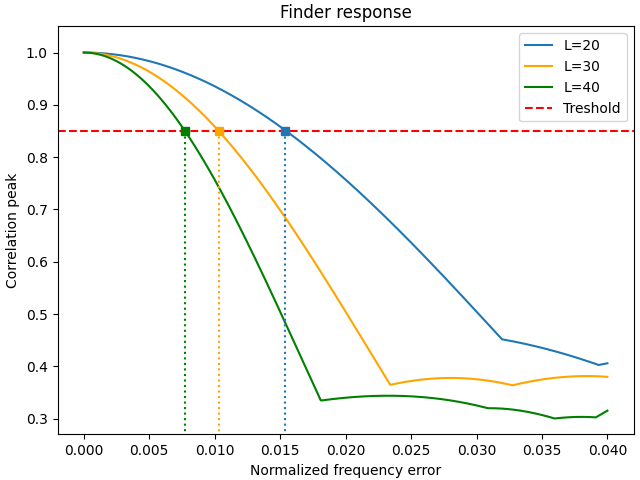
\includegraphics[width=\textwidth]{pics/finder_response.png}
\end{figure}

Увеличение длины преамбулы приводит к росту её энергии при фиксированной мощности передатчика, что повышает дальность обнаружения сигнала. Однако увеличение длины преамбулы также повышает вычислительную нагрузку и усложняет процедуру частотного поиска.

Таким образом, выбор длины преамбулы представляет собой компромисс между энергетическими характеристиками обнаружителя и вычислительной сложностью его реализации.

